\documentclass[11pt, a4paper]{article}
\usepackage[utf8]{inputenc}
\usepackage{mathpazo} % Palatino font
\usepackage{lineno}
\usepackage{setspace}
\usepackage{caption}
\usepackage{graphicx, subfig}
\usepackage{cite}
\usepackage{float} %so the graphs are not floating around after I put[H]
\usepackage[margin=2cm]{geometry}
\usepackage{indentfirst}
\usepackage{natbib} 

\begin{document}
\begin{spacing}{1.5}

\begin{titlepage} % Suppresses displaying the page number on the title page and the subsequent page counts as page 1
	\newcommand{\HRule}{\rule{\linewidth}{0.5mm}} % Defines a new command for horizontal lines, change thickness here
	
	\center % Centre everything on the page
	
	%------------------------------------------------
	%	Headings
	%------------------------------------------------
	
	\textsc{\LARGE Imperial College London}\\[2.5cm] % Main heading such as the name of your university/college
	
	\textsc{\Large Computational Method in Ecology and Evolution}\\[2.5cm] % Major heading such as course name
	

	%------------------------------------------------
	%	Title
	%------------------------------------------------
	
	\HRule\\[0.6cm]
	
	{\huge\bfseries Thermal Response Model Selection and Analysis is Dependent on the Studied Traits and Temperature Range}\\[0.4cm] % Title of your document
	
	\HRule\\[2.5cm]
	
	%------------------------------------------------
	%	Author(s)
	%------------------------------------------------
	
	\begin{minipage}{0.4\textwidth}
		\begin{center}
			\large
			\textit{Author: }
			\text{Danica Duan}\\
			\textit{CID: }
			\text{01790819}% Your name
		\end{center}
	\end{minipage}

	
	% If you don't want a supervisor, uncomment the two lines below and comment the code above
	%{\large\textit{Author}}\\
	%John \textsc{Smith} % Your name
	
	%------------------------------------------------
	%	Date
	%------------------------------------------------
	
	\vfill\vfill\vfill % Position the date 3/4 down the remaining page
	
	{\large\today} % Date, change the \today to a set date if you want to be precise

	 
	%----------------------------------------------------------------------------------------
	
	\vfill % Push the date up 1/4 of the remaining page
	Word Count: 2378

\end{titlepage}

%----------------------------------------------------------------------------------------


\linenumbers
\renewcommand\thesection{\arabic{section}}
\section{Keywords}
Microbial community; temperature; thermal response; carbon cycle; species interaction; microbial metabolism
\section{Introduction}

Temperature is a crucial factor for microbial metabolism, higher temperature could lead to the acceleration of activity rates, increasing growth rate and interactions, etc. However, most studies regarding microbial responses to temperature fluctuations were conducted on single strains or taxa level, forgoing the highly complex interactions within microbial communities. 

Microbes play a central role in Earth carbon cycling. Microbial carbon use efficiency (CUE) describes the ratio of carbon assimilation and carbon intake, which considers organic matter decomposition, biomass production and carbon loss through respiration and extracellular secretion of organic carbon \citep{bardgett2008microbial}. The general effect of global warming on CUE is difficult to predict since all processes mentioned above are related to microbial metabolism and enzyme reactions, which would all be impacted by temperature changes \citep{davidson2006temperature, smith2019community, gang2019meta} but at different degrees depending on their temperature sensitivity. 

Species interaction is of critical importance while considering microbial CUE, since cross-feeding activities could affect the distribution of carbon source through by-product secretion as secondary carbon sources, which could facilitate some species and release competitions. In this way, species interaction also plays a determinative role on community assembly and structure.

Microbial community composition and diversity are fundamental for a wide range of eco-functions, including the decomposition of organic matter \citep{liebich2007degradation, perveen2014priming}. The fundamental pattern of diversity shift with long-term and short-term temperature changes was not found, however was reported to display differently with regions(hotter or colder) and habitats \citep{zhou2016temperature, zhou2020meta, luo2019seasonal, gilbert2012defining}.

In this project, I propose to study the responses of mesophile (microbes best operate at moderate temperature range) bacterial communities to temperature fluctuations. I will address the following research questions: 1) How will bacterial carbon use efficiency be affected by changing temperature? 2) How will species interactions in bacterial community be affected by changing temperature? 3) Will bacterial diversity increase with warming? 

\section{Methods}
To understand species interactions and resource partitioning during community assembly under temperature impacts, I will 1) adapt consumer resource model \citep{goldford2018emergent} which simulates dynamics of individual species growth with resource assimilation, and cross-feeding interactions through a stoichiometric matrix which encodes the proportion of by-product secretion from substrate uptake; and the thermodynamic consumer resource model from \cite{marsland2019available} to include simulations on energy fluxes of microbial metabolism, stochastic colonization and competition. 2) add temperature impacts on bacterial metabolism into the system to investigate how are interactions and resource partitioning affected by temperature.

Microbial CUE can be analysed with carbon uptake, assimilation (growth) and carbon loss (leakage from the system) from the model; and the species diversity can be analysed as the number of species with abundance over zero at the end of model simulation.

\section{Anticipated outputs and outcomes}

Ideally, through predictions of temperature effects on species interaction during community assembly, the output will provide fundamental understandings of temperature impacts on bacterial community structure and carbon cycling function. This study will be filling the gaps of understanding community level temperature response and the temperature effects on bacterial community CUE.  

\section{Project feasibility}

\begin{figure}[H]
    \centering
    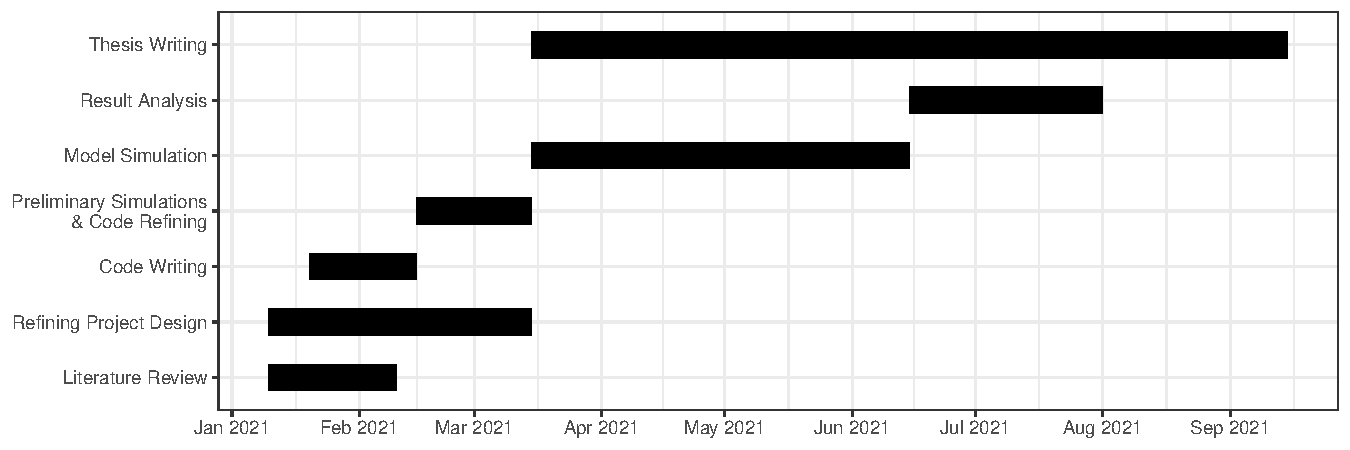
\includegraphics[scale = 0.74]{Gantt_chart.pdf}
    \caption{Gantt chart of the general project plan.}
    \label{fig:Gantt_chart}
\end{figure}

\section{Budget}

Computational project with free resources, no budget anticipated. 

\bibliographystyle{agsm}
\bibliography{Proposal}

\pagebreak

I have seen and approved the proposal and the budget. \\

Supervisor: Samraat Pawar\\

Signature: \\

Date: 23/12/2020
\end{spacing}
\end{document}
